\begin{tutorial}{A+B}

\medskip
\textit{Автор задачи: Михаил Путилин}
\medskip

\subsection*{Подзадача 1}
Первая подзадача решается перебором $n!$ перестановок.

\subsection*{Подзадача 2}
Каждый столбец можно охарактеризовать тремя параметрами (обозначим цифры в нём за $a_i$, $b_i$, $c_i$):
\begin{enumerate}
\item Есть ли в нём цифра ноль (это влияет на то, может ли он быть первым).
\item Требуется ли ему перенос из столбца справа, в зависимости от того, верно $(a_i+b_i) \mod 10=c_i$ или $(a_i+b_i+1) \mod 10=c_i$. Если ни одно из этих равенств не выполнено, то ответ $0$. Обозначим этот параметр $needCarry_i \in \{0,1\}$.
\item Создаёт ли этот столбец перенос через разряд. Это так, когда $a_i+b_i+needCarry_i \geq 10$. Обозначим этот столбец $makeCarry_i \in \{0,1\}$.
\end{enumerate}
Будем выбирать перестановку столбцов слева направо. Первым может идти столбец без нулей и не создающий переноса. Если после столбца $i$ идёт столбец $j$, то $needCarry_i=makeCarry_j$. Для последнего столбца $needCarry_i=0$. Получается граф, в котором нужно найти число гамильтоновых путей. Это можно сделать при помощи динамического программирования за $O(2^n n^2)$, решив, таким образом, вторую подзадачу.

\subsection*{Подзадачи 3 и 4}
\begin{center}
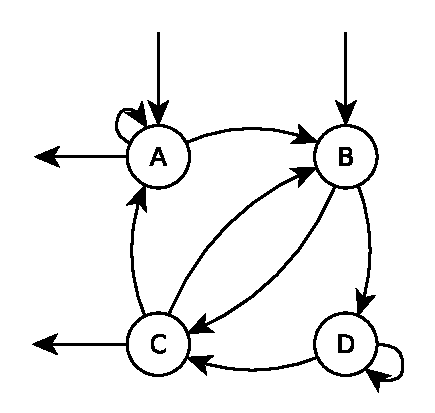
\includegraphics{tutor_graph.eps}
\end{center}
В полученном графе есть четыре вида вершин в зависимости от значений $needCarry_i$ и $makeCarry_i$. Обозначим эти виды следующим образом:
\begin{itemize}
\item Тип A: $needCarry_i=0$, $makeCarry_i=0$
\item Тип B: $needCarry_i=1$, $makeCarry_i=0$
\item Тип C: $needCarry_i=0$, $makeCarry_i=1$
\item Тип D: $needCarry_i=1$, $makeCarry_i=1$
\end{itemize}
На рисунке показано, какие рёбра есть в графе, а также какие вершины могут быть начальными и конечными.

Посчитать гамильтоновы пути в таком графе можно динамикой за $O(n^4)$: $d_x[A][B][C][D]$~--- число путей, которые заканчиваются в вершине вида $x$ и проходящие через соответствующее число вершин каждого вида. Это решает подзадачу 3.

Чтобы решить подзадачу 4, нужно учесть, что нельзя начинать со столбца с нулём. Это влияет только на базу динамики: в $d_A[1][0][0][0]$ и $d_B[0][1][0][0]$ нужно записать количество соответствующих столбцов, в которых нет нулей.


\subsection*{Подзадачи 5 и 6}
На любом пути в таком графе, который начинается в A или B, количество вершин вида B не более чем на один превосходит количество вершин вида C. Это позволяет сократить число состояний в динамике до $O(n^3)$, решив, таким образом, подзадачи 5 и 6.

\subsection*{Подзадача 7}
Обозначим за $A$, $B$, $C$, $D$ количество вершин каждого вида. Любой интересующий нас путь выглядит следующим образом:

$$\_ B \_ C \_ B \_ C \_ B \_ C \dots B \_ C \_$$

При этом вершины A расположены в промежутках перед B, а также в последнем. Вершины D расположены в промежутках после B. Кроме того, если $B \neq C$, то ответ 0.

Если $B=C=0$ и $D>0$, то ответ 0. Если $B=C=0$ и $D=0$, то ответ $A!$.

Если $B=C>0$, то ответом будет произведение следующих чисел:
\begin{enumerate}
\item Количество способов расставить вершины B по местам: $B!$
\item Количество способов расставить вершины C по местам: $B!$
\item Количество способов расставить $A$ вершин в $B+1$ промежуток с учётом порядка: $\frac{(A+B)!}{B!}$.
\item Количество способов расставить $D$ вершин в $B$ промежутков с учётом порядка: $\frac{(D+B-1)!}{(B-1)!}$.
\end{enumerate}

Ответ равен $(A+B)!(D+B-1)!B$. Это решение за $O(n)$ проходит подзадачу 7.

\subsection*{Подзадача 8}
Осталось учесть, что среди вершин вида A и B может быть сколько-то вершин, с которых нельзя начинать (столбцы с нулями). Обозначим эти количества за $A_0$ и $B_0$.

Как и в прошлой подзадаче, если $B=C=0$ и $D>0$, то ответ 0. Если $B=C=0$ и $D=0$, то ответ $(A-1)! \cdot (A-A_0)$.

Далее $B=C>0$. Сначала отдельно посчитаем:
\begin{itemize}
\item $ans_B$~--- число путей, которые начинаются с вершины вида B. Это означает, что промежутков, в которые можно ставить вершины A, не $B+1$, а $B$. Тогда $ans_B=B! \cdot B! \cdot \frac{(A+B-1)!}{(B-1)!} \cdot \frac{(D+B-1)!}{(B-1)!} = (A+B-1)!(D+B-1)!B^2$
\item $ans_A$~--- число путей, которые начинаются с вершины вида A. $ans_A = (A+B)!(D+B-1)!B-ans_B$
\end{itemize}

Ответ равен $ans_A \cdot \frac{A-A_0}{A} + ans_B \cdot \frac{B-B_0}{B}$.

\end{tutorial}
